\section{Anexos}
\subsection{Características de un transformador}

\begin{itemize}
    \item \textbf{Núcleo}: Su función principal consiste en retener ese flujo magnético de manera contenida para prevenir las pérdidas ocasionadas por las corrientes de Foucault. Por lo general, está compuesto por láminas de metal apiladas, si bien su material y forma pueden variar según el tipo de transformador \cite{ferrovial_stem}.
    \item \textbf{Bobinas}: Normalmente están constituidas por hilos de cobre que se enrollan alrededor del núcleo y son responsables de generar el cambio de voltaje. El número de vueltas o espiras en cada bobina guarda una relación directa con el voltaje; a mayor cantidad de espiras, mayor es el voltaje producido. Un transformador, como mínimo, posee dos bobinas: la primaria, por la cual entra la corriente y se conoce como devanado primario, y la secundaria, por donde sale la corriente. La cantidad de espiras en la bobina primaria corresponde al voltaje de entrada, mientras que la cantidad de espiras en la bobina secundaria está asociada al voltaje de salida del transformador \cite{ferrovial_stem}.
    \item \textbf{Aislante}: los elementos de un transformador se encuentran separados entre sí por un aislante, debido a que cada uno de ellos tiene tensiones diferentes. En transformadores de alta tensión, es común emplear una capa de papel impregnado en aceite mineral para aislar el núcleo de los devanados, así como para separar los propios devanados. Las espiras adyacentes suelen estar aisladas mediante una fina capa de laca de cobre, mientras que aquellas que no son consecutivas pueden contar con aislamiento de laca o papel, según las necesidades específica \cite{ferrovial_stem}.
\end{itemize}

\subsubsection{Transformador de Corriente}

Un transformador de corriente consta de un devanado primario, un núcleo y un devanado secundario. A pesar de que comparten principios físicos similares, las especificaciones entre un transformador de corriente y uno de tensión difieren debido a los requisitos particulares de sus aplicaciones. El transformador de corriente está específicamente diseñado para mantener una relación precisa entre las corrientes en sus circuitos primario y secundario dentro de un rango definido \cite{wiki_transformador_corriente}.

La corriente alterna en el devanado primario genera un campo magnético variable en el tiempo en el núcleo, induciendo a su vez una corriente alterna en el devanado secundario. Es importante destacar que la conexión del transformador de corriente no afecta al circuito primario. La precisión de este tipo de transformador depende del acople entre el primario y el secundario, asegurando que la corriente secundaria sea proporcional a la corriente primaria en un rango más amplio de corriente. La corriente en el secundario se obtiene dividiendo la corriente en el primario entre el número de vueltas en el devanado secundario \cite{wiki_transformador_corriente}.
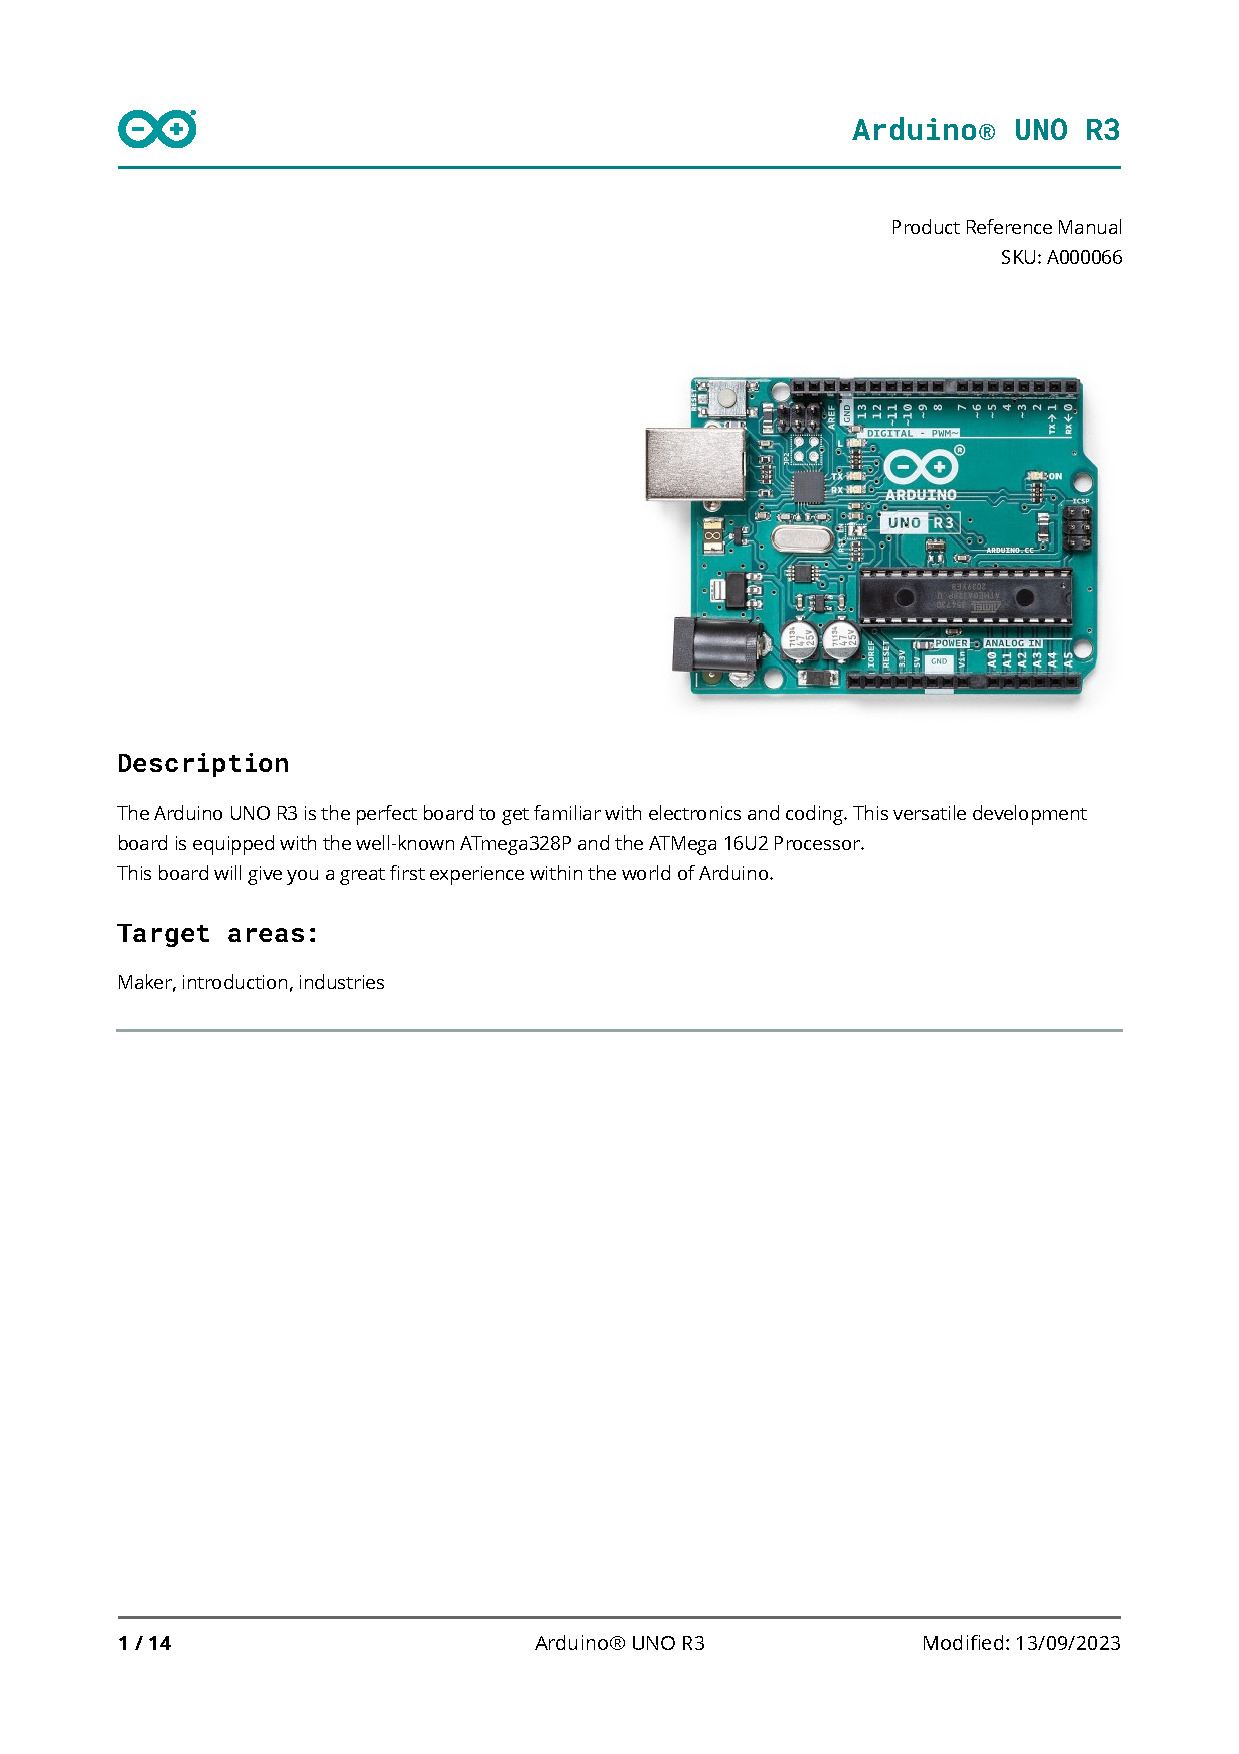
\includepdf[pages={1-10}]{Documentos/Arduino.pdf}
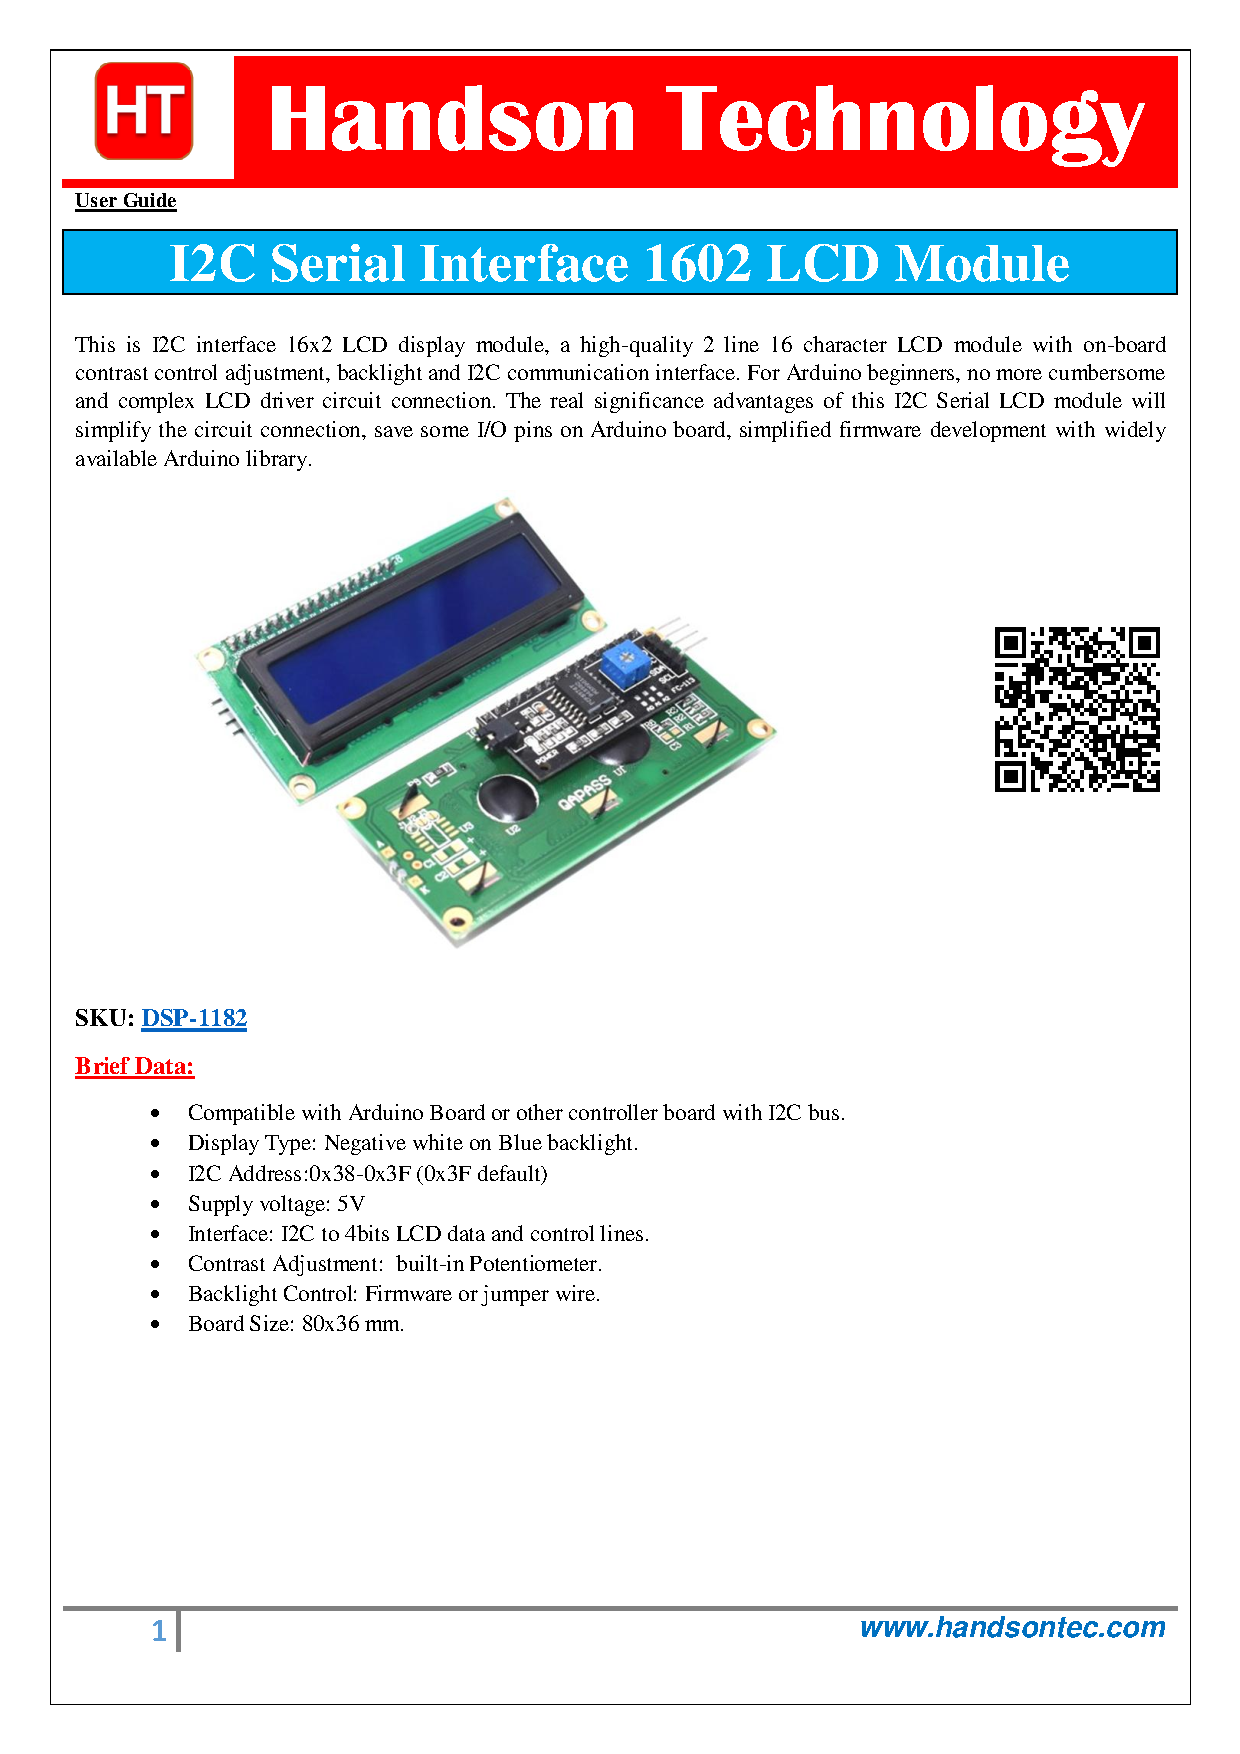
\includepdf[pages={1-3}]{Documentos/i2c_lcd.pdf}
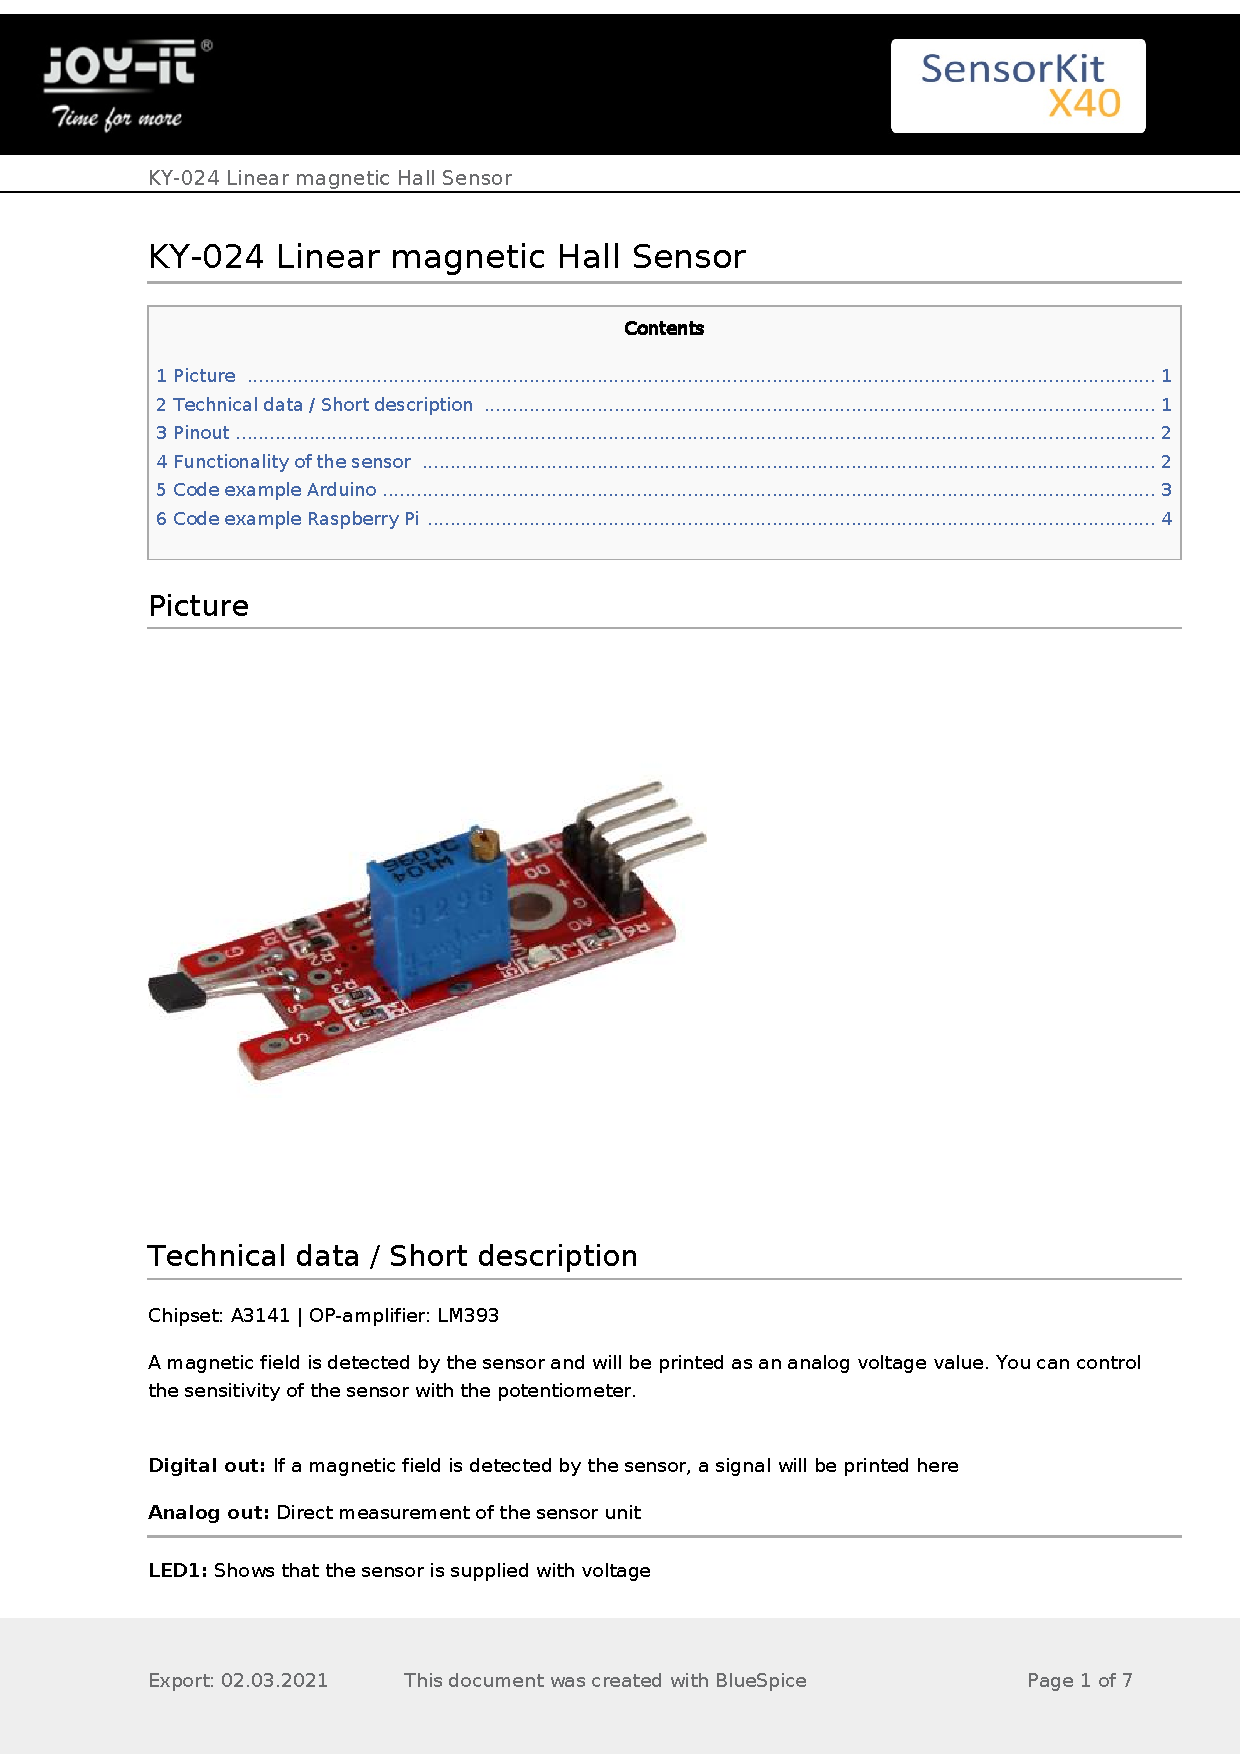
\includepdf[pages={1-3}]{Documentos/ModuleHall_KY-024.pdf}
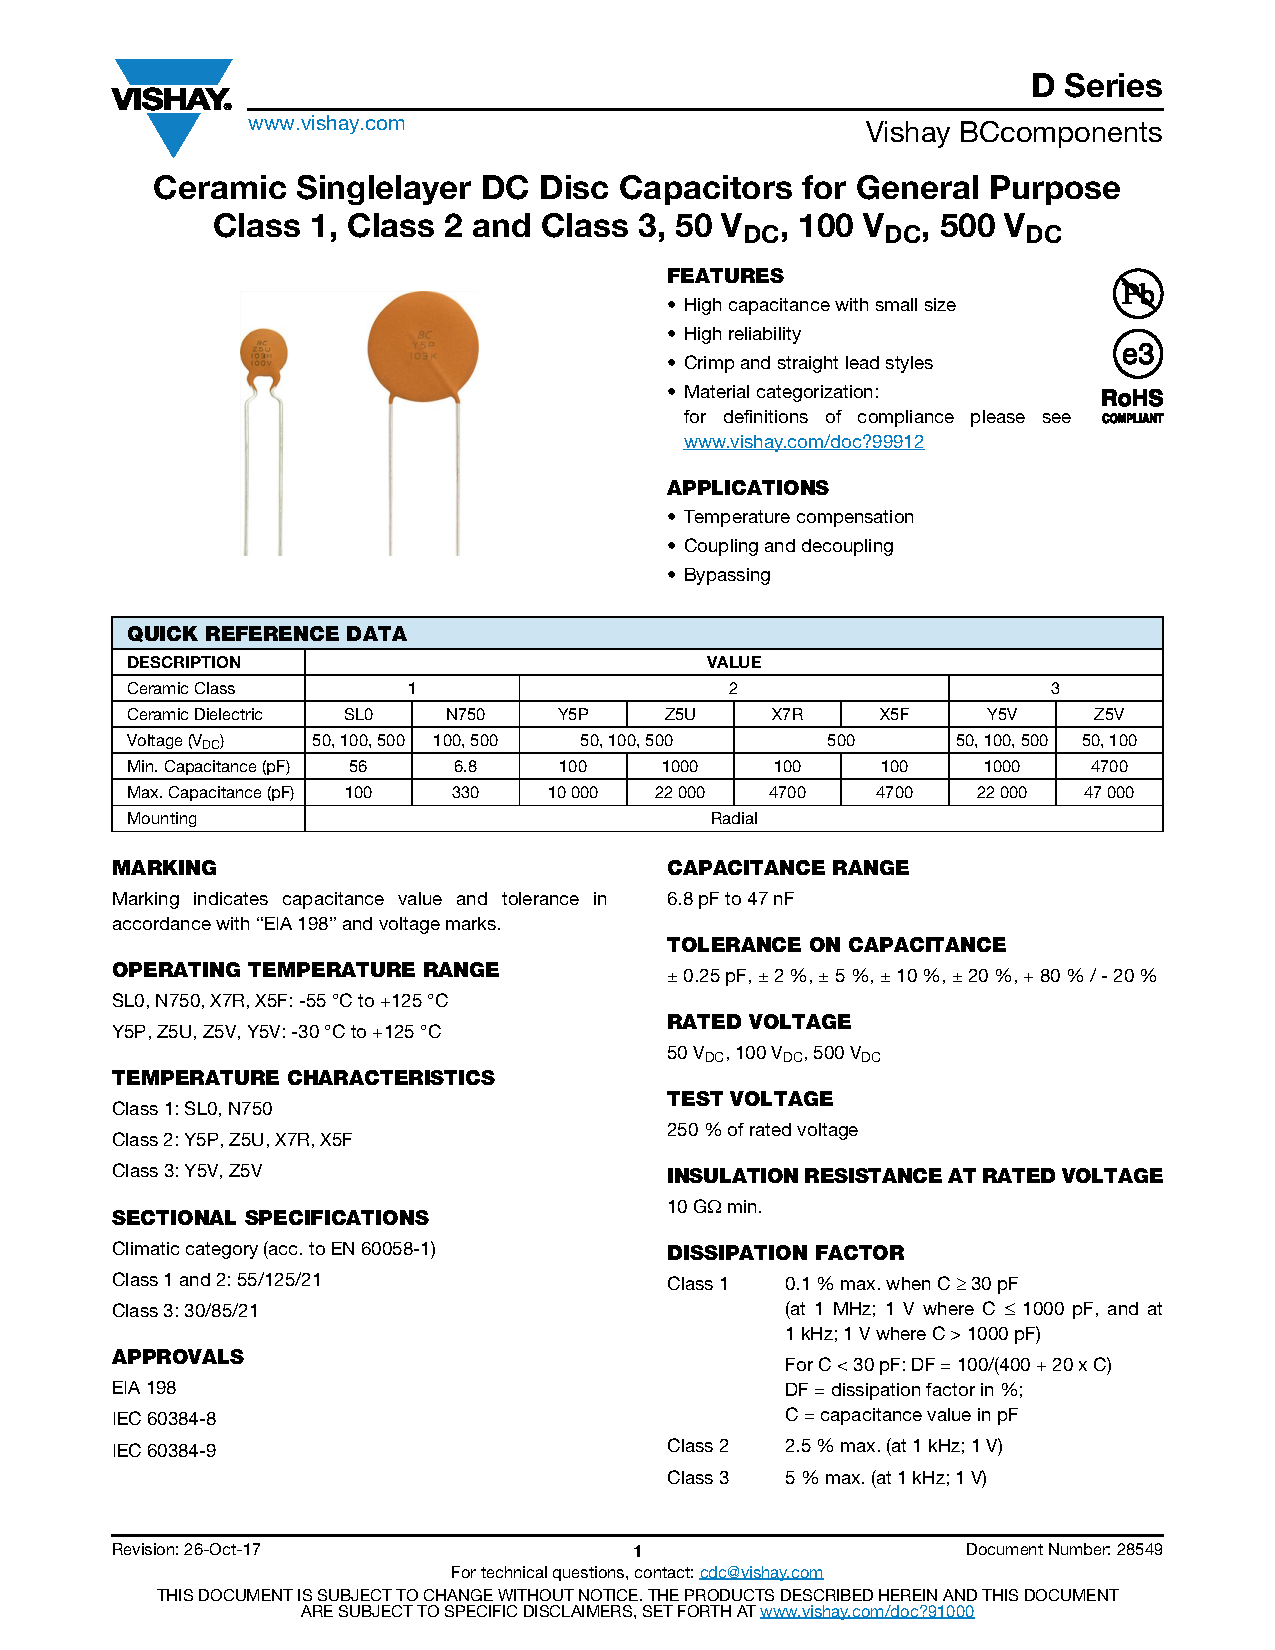
\includepdf[pages={1}]{Documentos/capacitor.pdf}
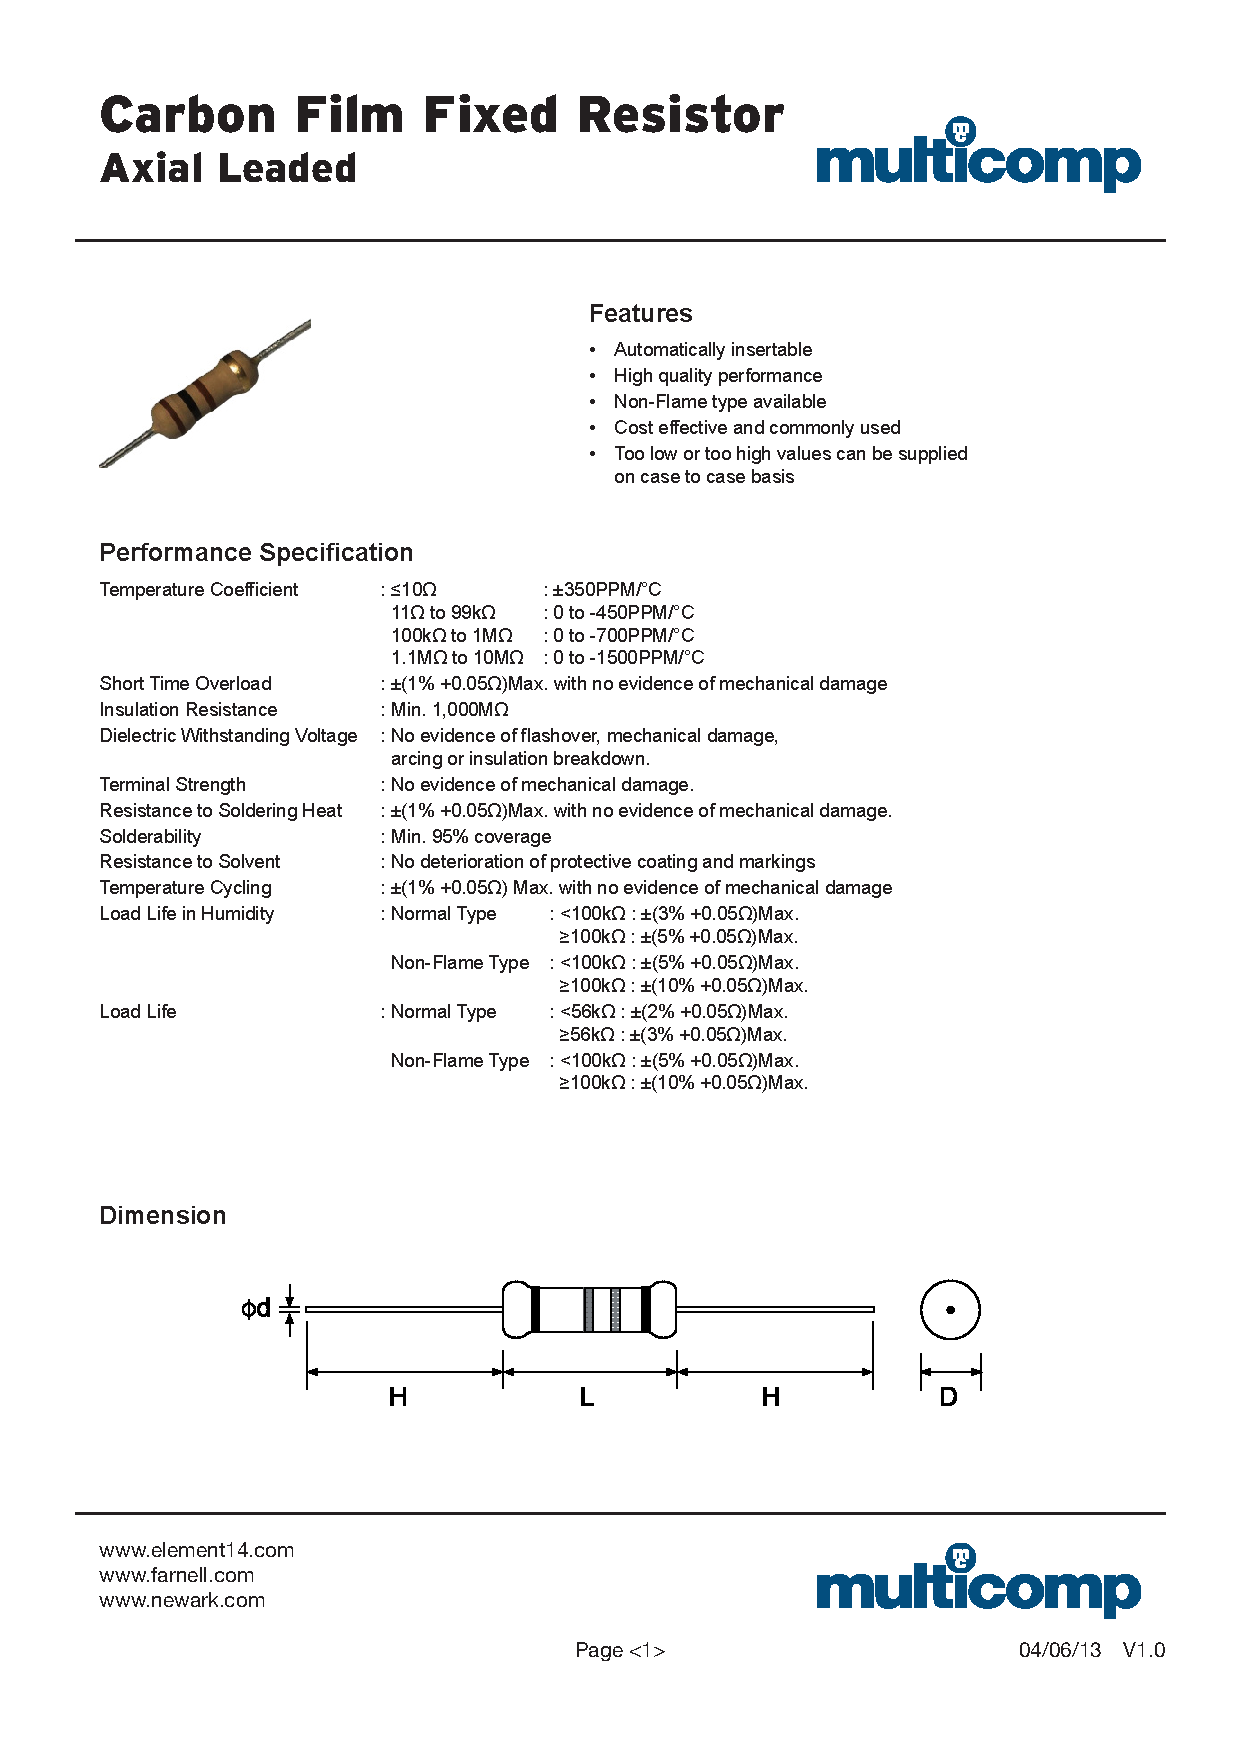
\includepdf[pages={1}]{Documentos/resistor.pdf}

  
  